\documentclass[12pt]{article}
\usepackage[margin=1in]{geometry}
\usepackage{setspace}
\usepackage{hyperref}
\usepackage{mathpazo}
\usepackage{amsmath}
\usepackage{graphicx}

\title{Inequality and the Labor Content of Consumption}
\author{}
\date{}

\begin{document}
\maketitle
\doublespacing


We define three matrices to map consumption by income group to the labor incomes it generates across the income distribution.

\paragraph{1. Consumption allocation matrix $A$}  
Let $A \in \mathbb{R}^{I \times K}$ be given by
\[
A =
\begin{bmatrix}
a_{11} & a_{12} & \cdots & a_{1K} \\
a_{21} & a_{22} & \cdots & a_{2K} \\
\vdots & \vdots & \ddots & \vdots \\
a_{I1} & a_{I2} & \cdots & a_{IK}
\end{bmatrix},
\]
where rows $i=1,\dots,I$ index \emph{income percentile groups} of consumers and columns $k=1,\dots,K$ index \emph{industries producing goods and services}.  
Element $a_{ik}$ denotes the share of consumption expenditure that group $i$ spends on industry $k$'s output.

\paragraph{2. Input-Output matrix $L$}  
Let $B \in \mathbb{R}^{K \times K}$ be the input–output ``use'' matrix (transposed from its standard format in National Accounts). In this matrix, $b_{kl}$ is the share of industry $k$'s gross output (i.e., total sales revenue) that they spend on inputs from industry $l$. Note that the rows will sum to less than one, because gross output is spent not only on intermediate inputs, but also on payments to labor, taxes, and net operating surplus (``payments to capital'').

The Leontief inverse of this matrix, if it exists, is
\[
L = (I_K - B)^{-1} =
\begin{bmatrix}
\ell_{11} & \ell_{12} & \cdots & \ell_{1K} \\
\ell_{21} & \ell_{22} & \cdots & \ell_{2K} \\
\vdots & \vdots & \ddots & \vdots \\
\ell_{K1} & \ell_{K2} & \cdots & \ell_{KK}
\end{bmatrix},
\]
where both rows and columns index industries.  
Element $\ell_{kl}$ gives the total (direct and indirect) inputs from industry $l$ purchased by industry $k$.

\paragraph{3. Distributional labor share matrix $D$}  
Let $D \in \mathbb{R}^{K \times I}$ be given by
\[
D =
\begin{bmatrix}
d_{11} & d_{12} & \cdots & d_{1I} \\
d_{21} & d_{22} & \cdots & d_{2I} \\
\vdots & \vdots & \ddots & \vdots \\
d_{K1} & d_{K2} & \cdots & d_{KI}
\end{bmatrix},
\]
where rows index industries and columns index income percentile groups of \emph{workers}.  
Element $d_{kj}$ denotes the share of labor compensation in industry $k$ accruing to workers in income decile $j$.

\paragraph{4. Mapping consumption to labor incomes}  
Multiplying these matrices yields
\[
M = A \, L \, D,
\]
where $M \in \mathbb{R}^{I \times I}$ has element $m_{ij}$ equal to the share of consumption expenditure by income percentile group $i$ that ultimately accrues as labor income to income percentile group $j$, after accounting for inter-industry linkages and the distribution of labor compensation within industries.

\section*{Input-output linkages over time}
Input output tables are obtained from the BEA. ``Use'' tables, producer pricing, before redefinitions.\footnote{The IO tables first measure each industry's purchase from each other industry; they then redefine these purchases to get each industry's purchases of each sectoral type of \emph{commodity}. We use the former, before redefinitions - because this is the only table that's collected constantly over time 1963-2023, but I think it's also what we want.} We define 56 industries constantly defined 1963-2023. Purchases are taken as shares of total industry output.

A dashboard visualizing these matrices over time is \href{https://martin-bernstein.github.io/LCC/figures/exploration/IO-matrices/IO_matrix_dashboard.html}{here}.

To better understand the changes in this matrix over time, we can compute each industry's ``eigenvector centrality.'' In the IO matrix $B$, where $b_{kl}$ is the share of industry $k$'s gross output that they spend on inputs from industry $l$, then one natural measure of each industry $l$'s centrality would be the vector $\mathbf c$ that satisfies:
\[
\lambda c_l = \sum_{k\neq l} b_{kl} c_k
\]
That is, industry $l$ is more ``important'' if many other ``important'' industries $k$ spend a lot of their revenue on industry $l$'s output. In matrix notation, if the above measure holds for all industries then $\lambda\mathbf c = B' \mathbf c$, so $\mathbf c$ is an eigenvector of the matrix $B'$ with eigenvalue $\lambda$. Linear algebra guarantees that the largest eigenvalue $\lambda$ will be positive and have an eigenvector with all positive values (up to scaling), so the eigenvector of that largest eigenvalue is taken to be the centrality measure.

Computing this eigenvector in each year gives figure \ref{eigcent}. The figure is intuitive: the centrality of agriculture and manufacturing sectors were high in 1960 and declined quickly to 1980; the centrality of insurance, real estate, professional/business/technical, and administrative services has risen quickly since 1980.

\begin{figure}\caption{Eigenvector centrality of industries over time}\label{eigcent}
    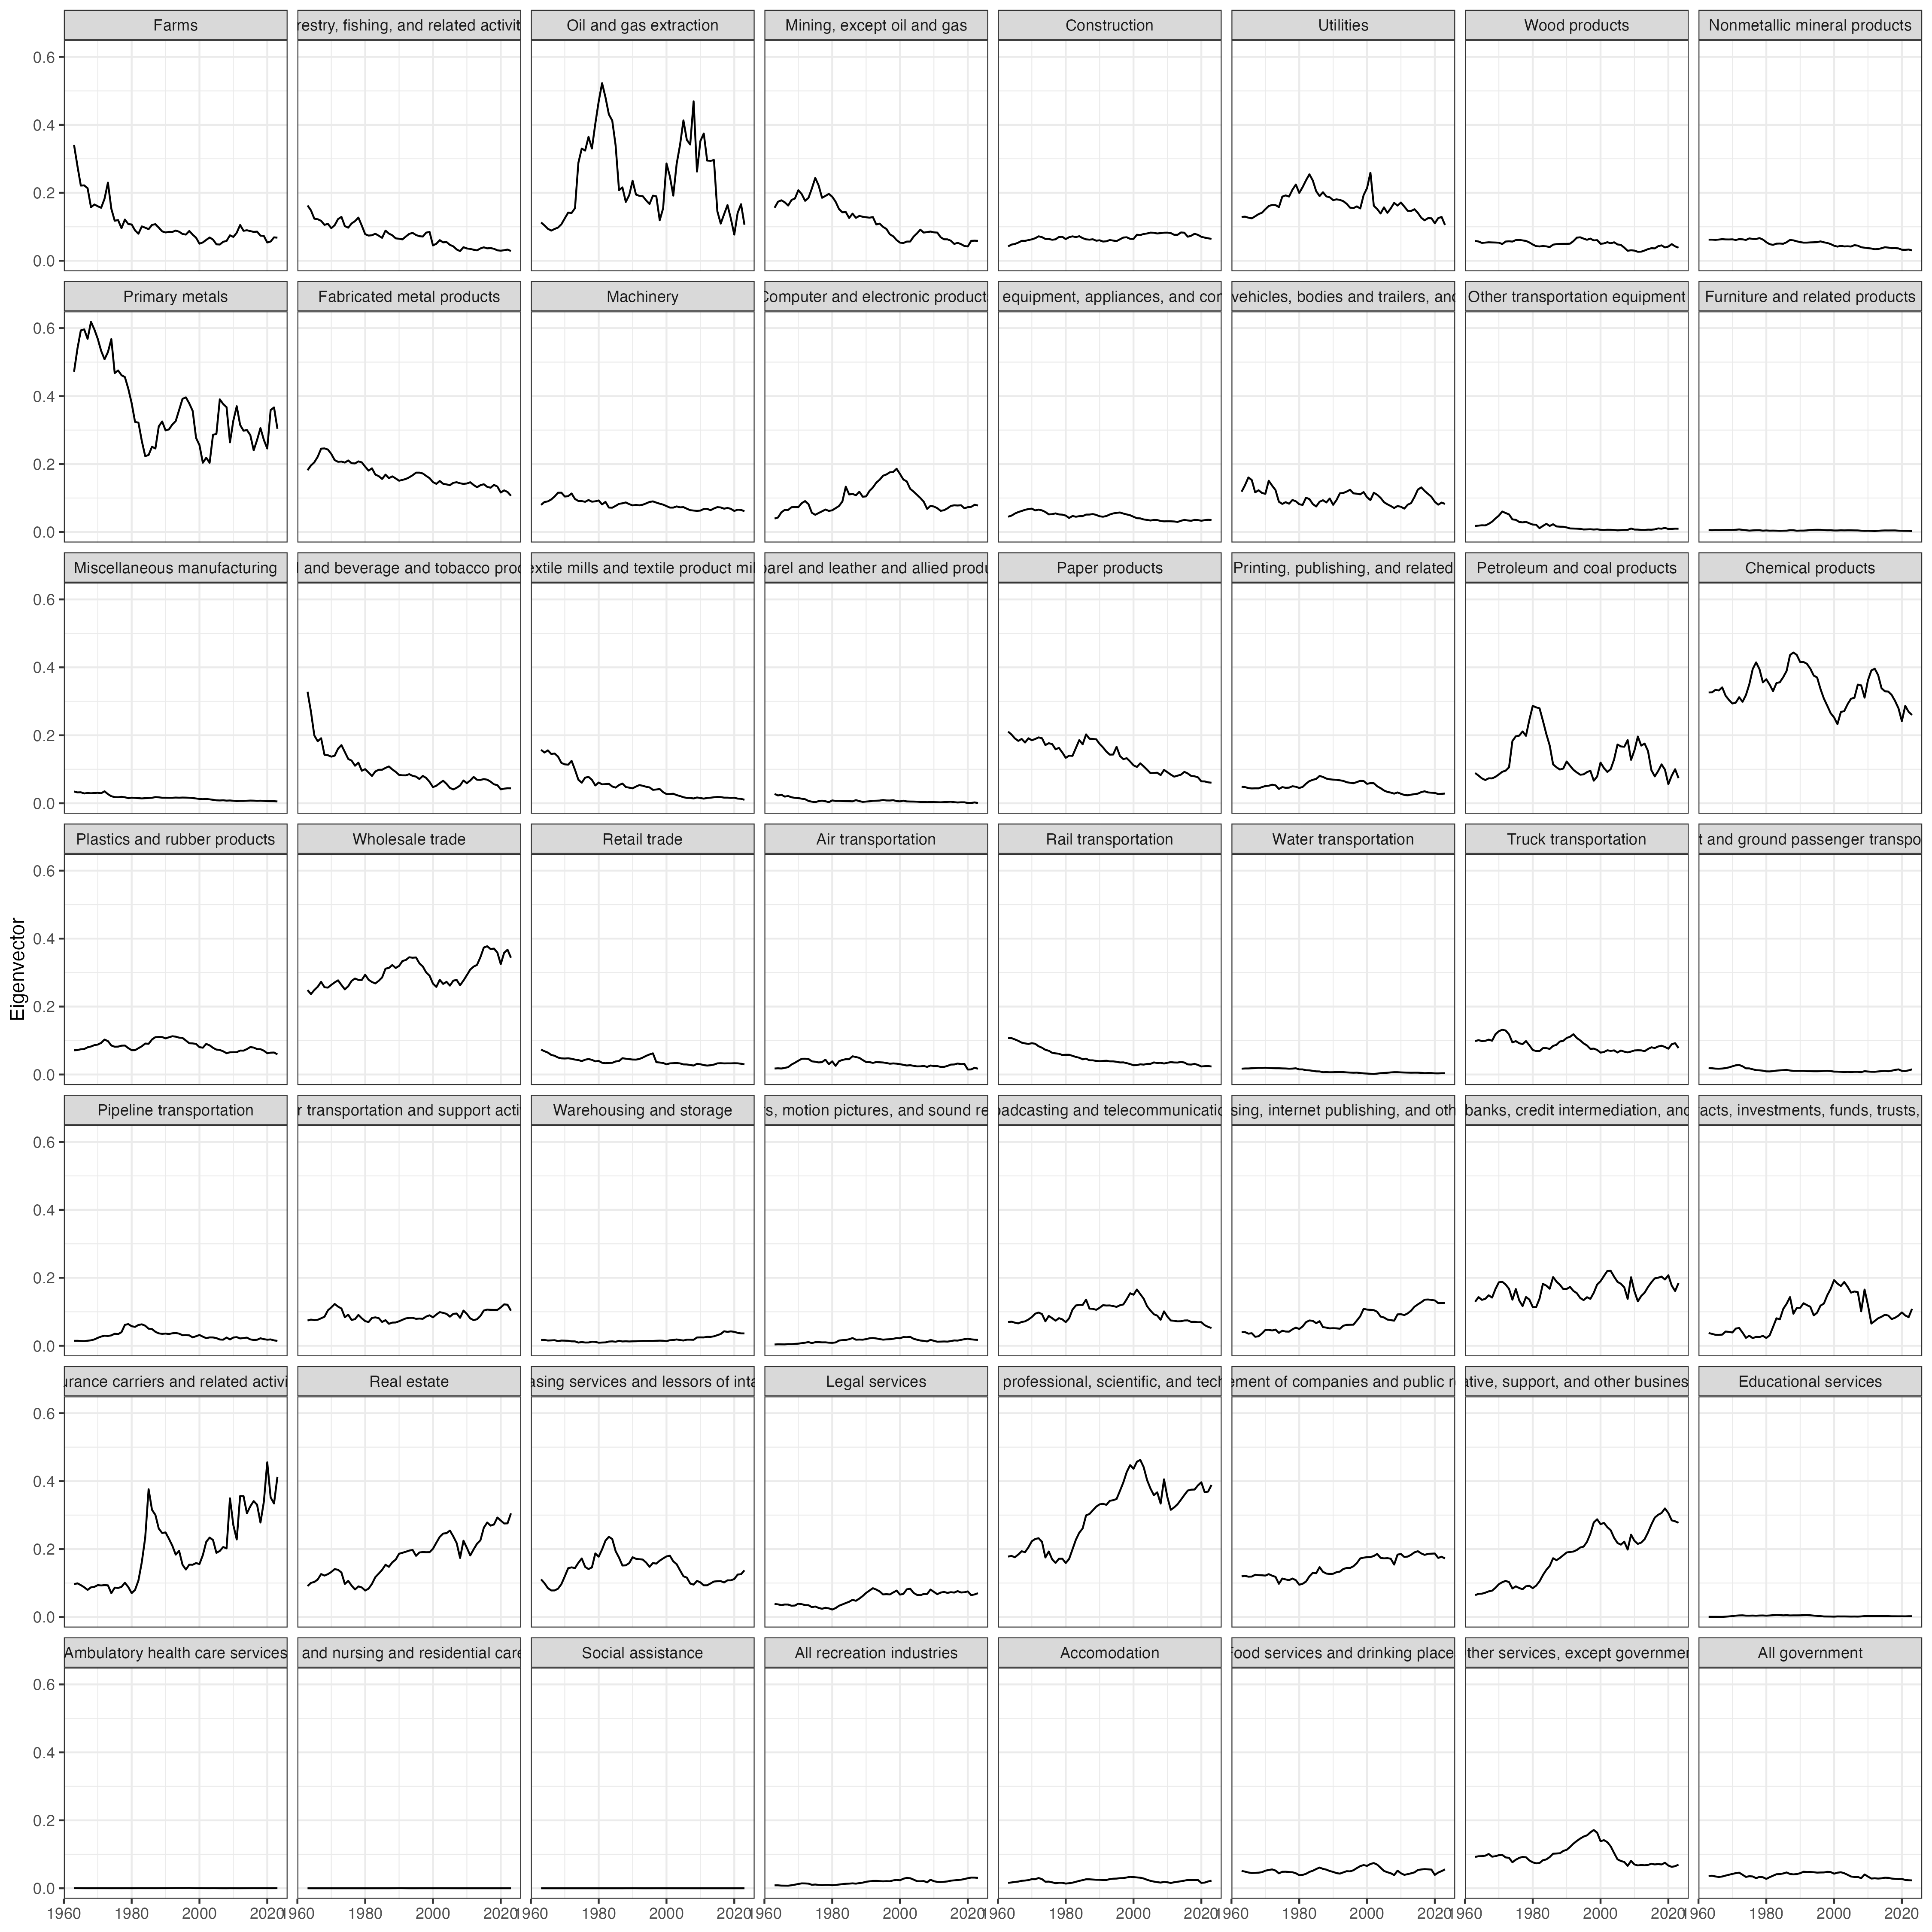
\includegraphics[width=\textwidth]{../figures/exploration/IO-matrices/industry_eigenvectors.png}
\end{figure}

\section*{Industry payments to factors}
The matrix $B$ is measured with input purchases per total output. To finish allocating industries' revenues, we need to measure their payments to labor and to capital, as the remaining shares of total output. In National Accounts, ``aggregate total output`` is ``gross output,'' which is decomposed into value added and intermediate inputs. Value added is payments to labor, net payments of taxes, and ``gross operating surplus'' Gross operating surplus can further be decomposed into net operating surplus and consumption of fixed capital (a measure of depreciation). Figure \ref{godecomp} measures these shares over time. Payments to capital (NOS and CPC) have risen, while payments to labor, intermediate inputs, and the government have fallen somewhat.

\begin{figure}\centering\caption{Aggregate gross output, decomposed}\label{godecomp}
    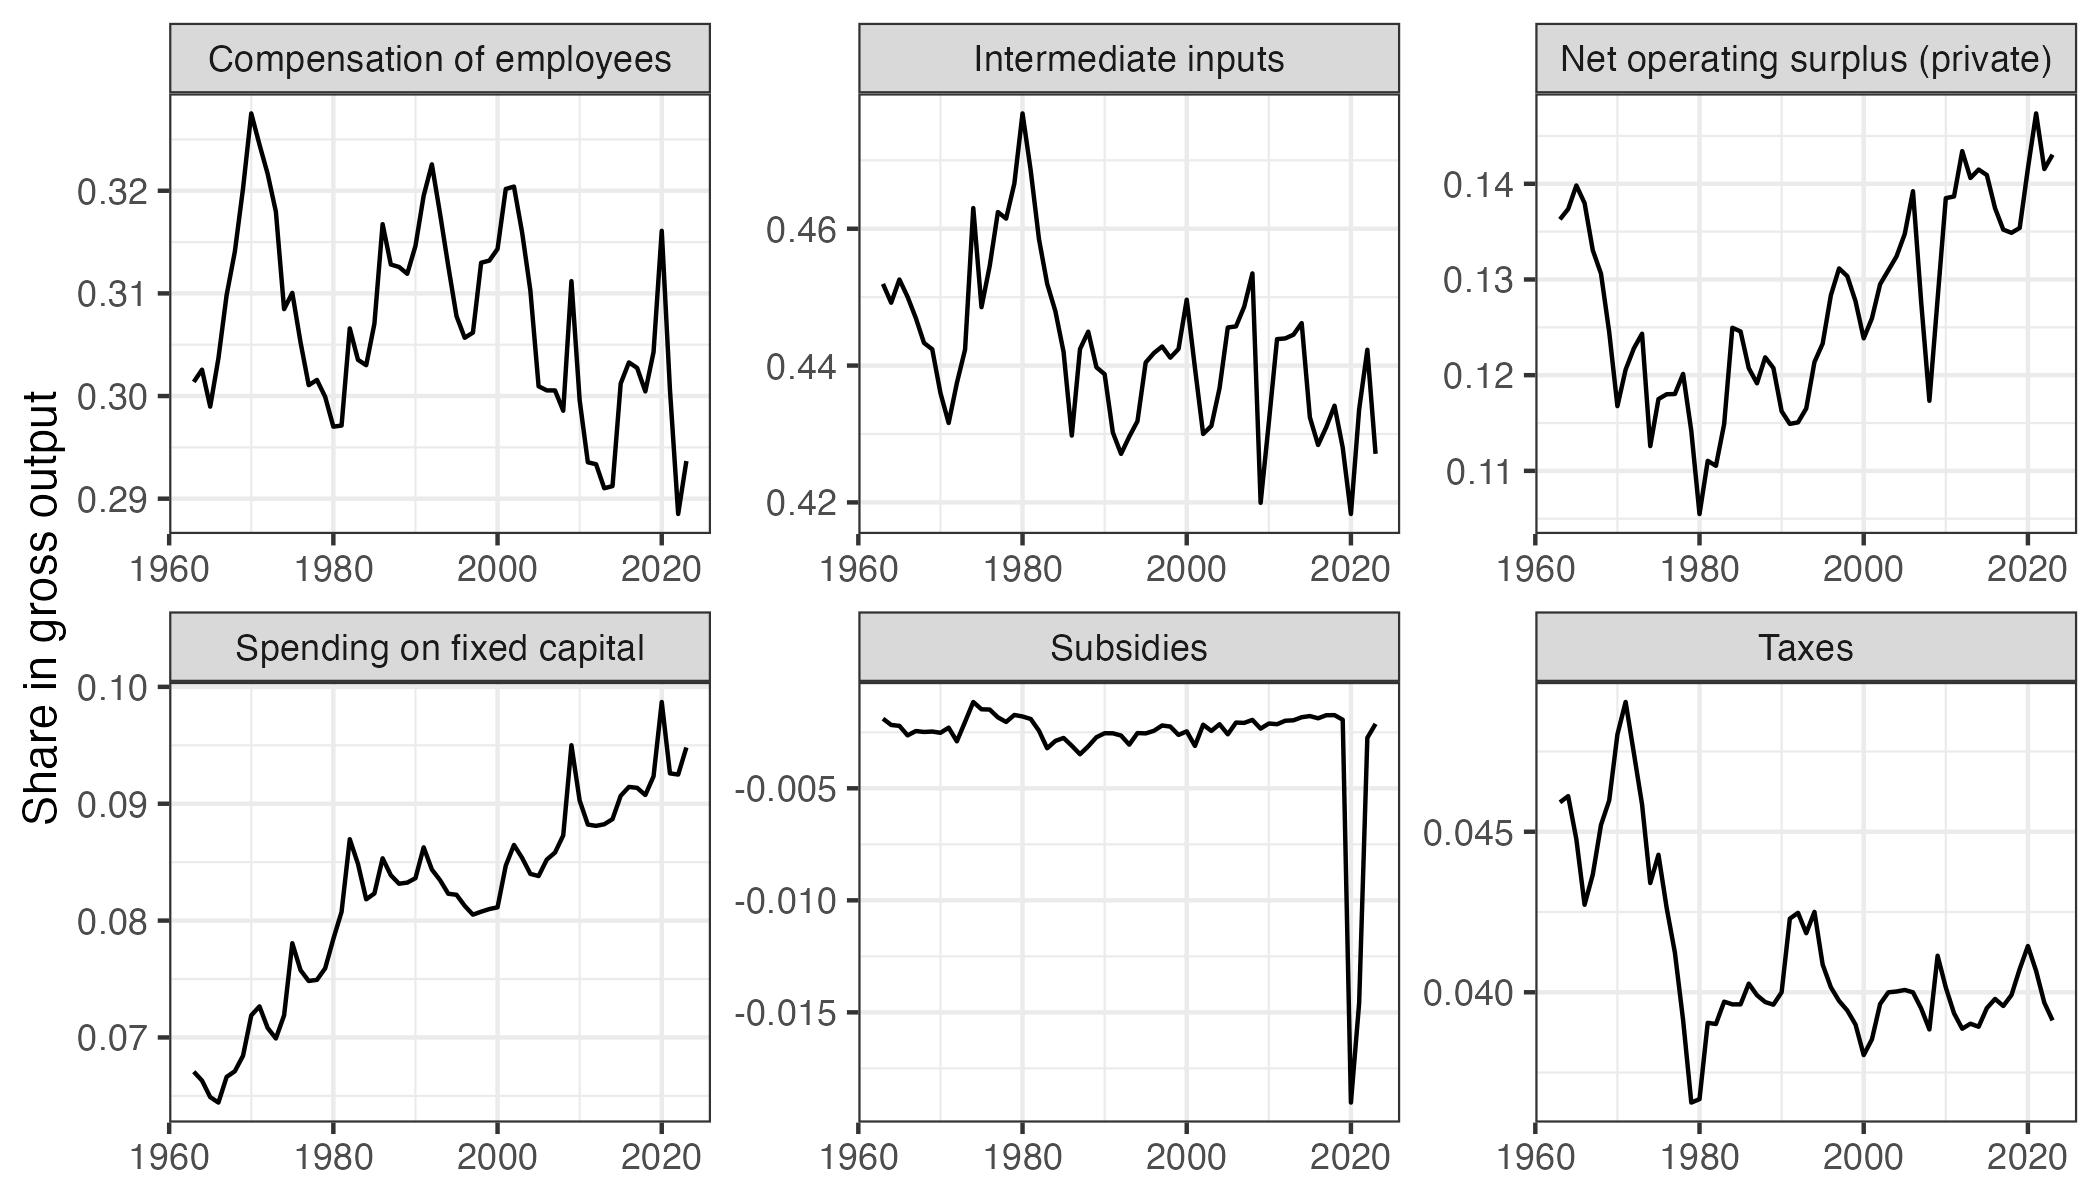
\includegraphics[width=.7\textwidth]{../figures/exploration/IO-matrices/aggregate_GO decomposition.png}
\end{figure}

The BEA National Accounts' GDP-by-industry KLEMS tables let us do this per industry. Using the same 56 industries we defined for the IO tables, KLEMS decomposes gross output into VA and intermediate inputs from 1929-2023, and then decomposes VA into payments to labor, taxes, and gross operating surplus from 1987-2023. To extend the data back to 1963, we take the shares of labor, taxes, and GOD in VA in 1987 and apply those to VA back to 1963. The result is figure \ref{ind_godecomp}. Then, the share of output paid to labor can be used to construct the matrix $D$.

\begin{figure}\caption{Industry-level decomopsition of gross output}\label{ind_godecomp}
    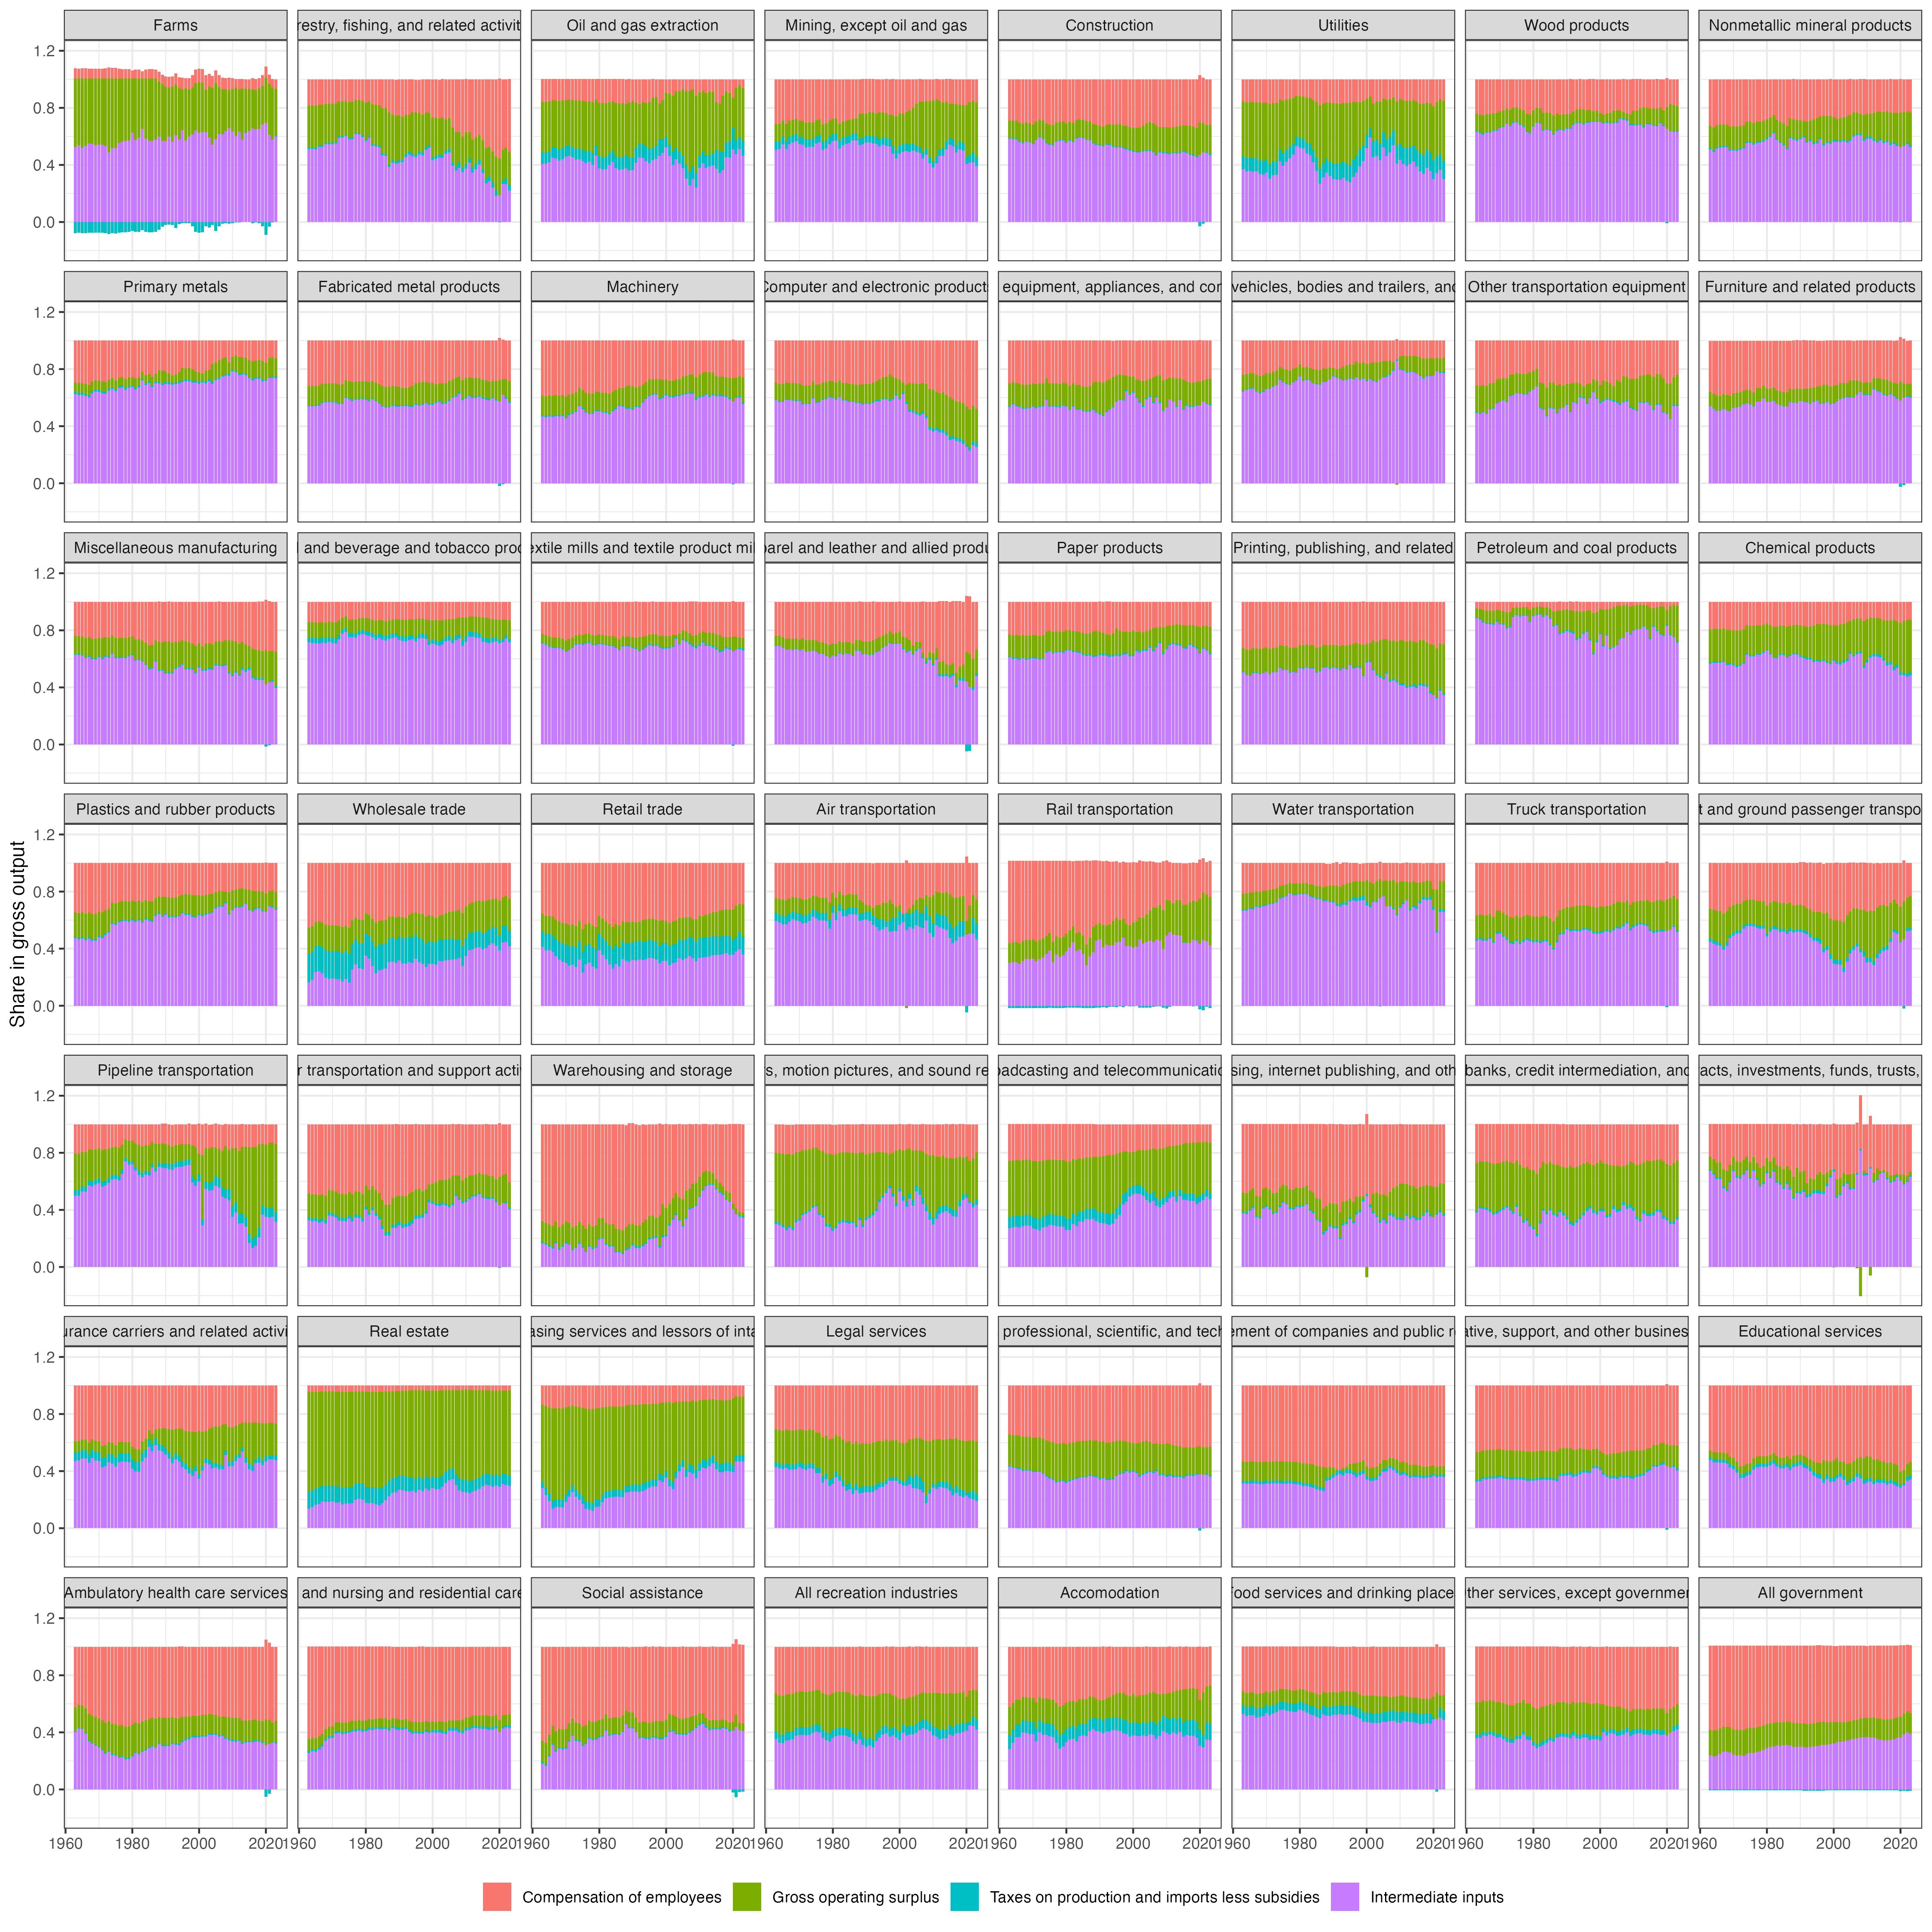
\includegraphics[width=\textwidth]{../figures/exploration/IO-matrices/GO = wL + GOS + T + M_with_imputation.png}
\end{figure}

\end{document} 
